%--------------------------------------------------------------------------------------------------
%
\chapter{Applications to Cluster Linking}\label{chap:applications}
%--------------------------------------------------------------------------------------------------

In online media streams -- particularly news articles -- there is often duplication of reporting,
different viewpoints or opinions, all centering around a single event. Typically each event is covered by many articles
and the question we address is how to find all the articles in different languages that are reporting on the same event.
The current chapter describes an application of the cross-lingual similarity presented in Chapter~\ref{chap:crosslingual}
to cross-lingual cluster linking. The application is relevant for monitoring global news in multiple languages.
Presented in the current chapter is our original approach to cross-lingual cluster linking,
which was published in~\cite{rupnikJAIR}. The main idea in our approach is to combine
semantic information extraction with cross-lingual document analysis, which we proved to be
effective in~\cite{Belyaeva201564}. There we used a simpler set of features to
decide which clusters to link and put greater emphasis on the manual evaluation of the quality.

To prepare the ground for the discussion of the cross-lingual approach, we will first
describe how \emph{events} are defined for our purposes and
sketch a general approach to event tracking in a monolingual setting.

The term event is vague and ambiguous, but for the practical purposes, we define
it as ``any significant happening that is being reported about in the media''.
Examples of events would include shooting down of the Malaysia Airlines plane over
Ukraine on July 18th, 2014 (see Figure~\ref{fig:event2}) and HSBC's admittance of
aiding their clients in tax evasion on February 9th, 2015. Events such as these are
covered by many articles and the question is how to find all the articles in
different languages that are describing a single event. Generally, events are more
specific than general themes as the time component plays an important role --
for example, the two wars in Iraq would be considered as separate events.

\begin{figure}
\centering
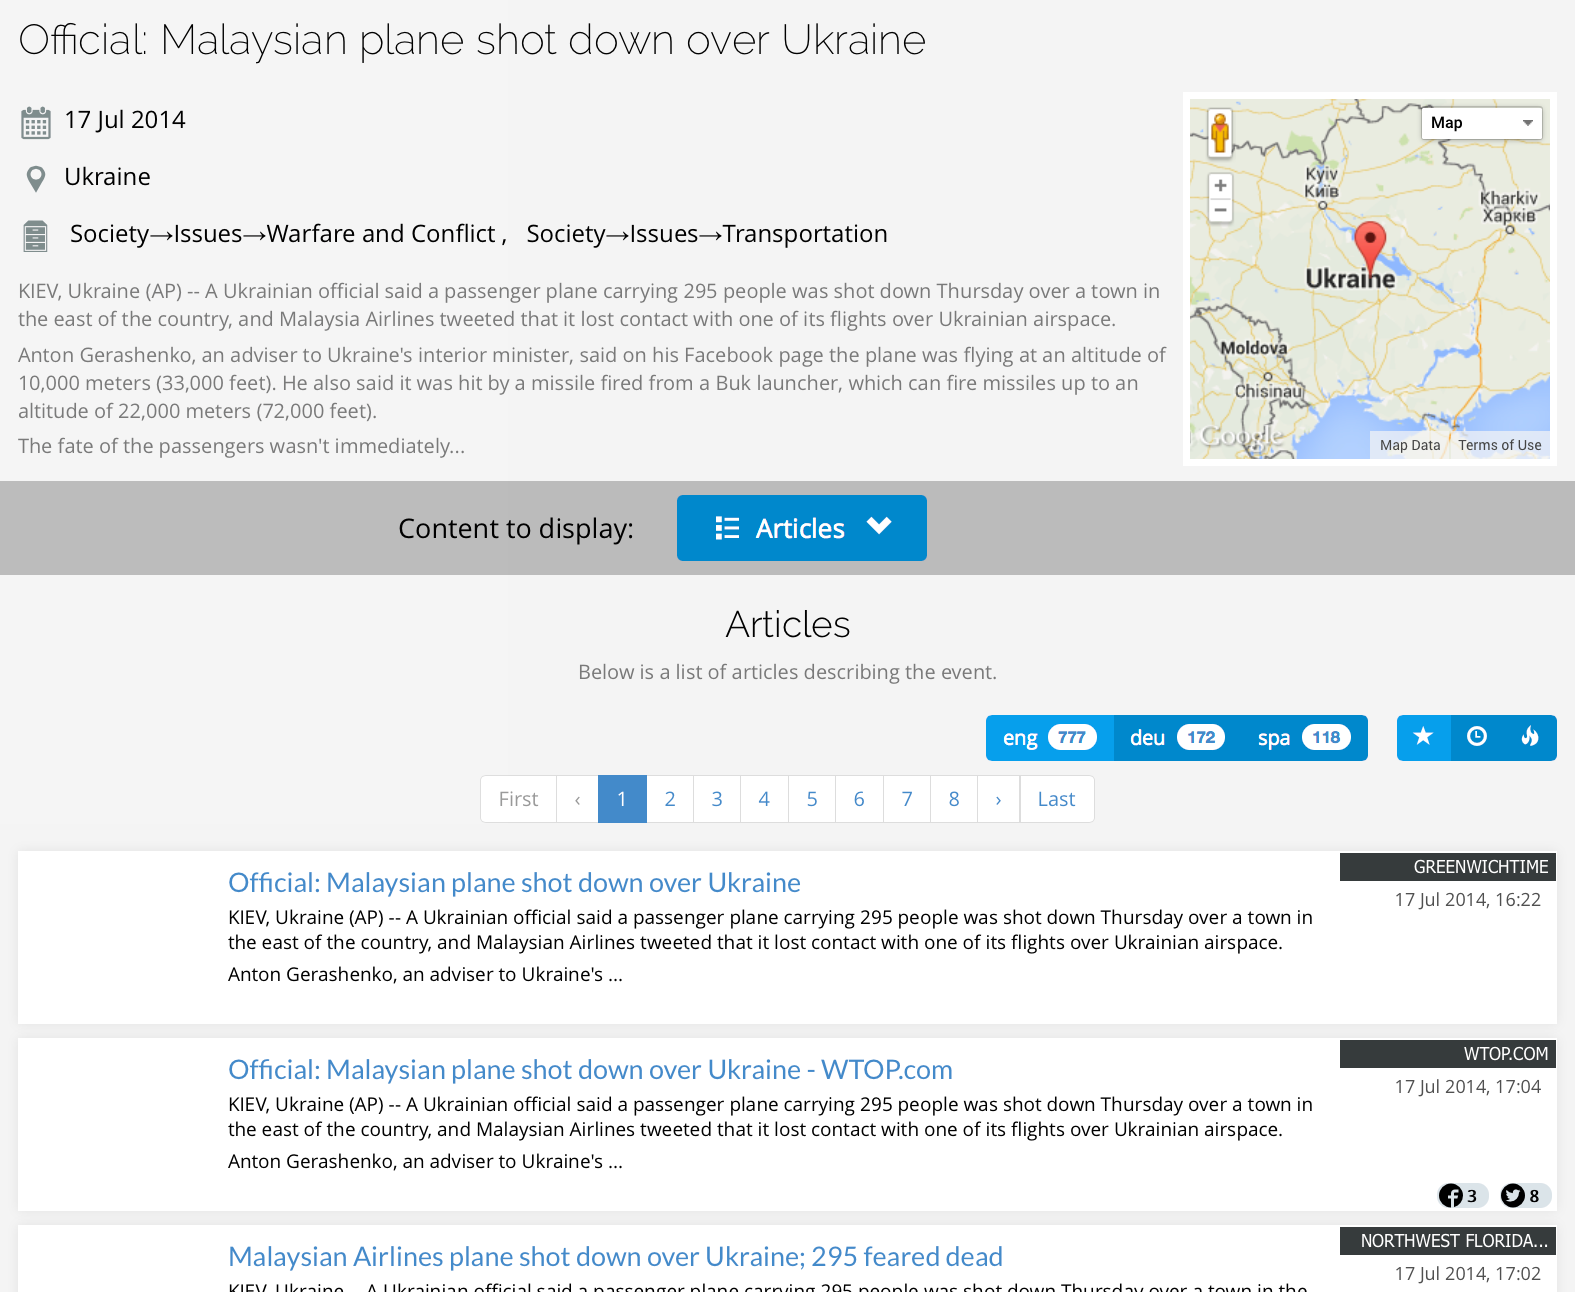
\includegraphics[width=1\textwidth]{figures/events2.png}
\caption[An example of an event]{Events are represented by collections of articles about an event, in
this case the Malaysian airliner which was shot down over Ukraine. The results shown in the figure can be obtained using the query \url{http://eventregistry.org/event/997350\#?lang=eng\&tab=articles}. The
content presented is part of the Event Registry system.}
\label{fig:event2}
\end{figure}


We take a pragmatic approach where the events are \textbf{identified} as the clusters
discovered by stream clustering algorithm that is designed to cluster
news articles together if their content is similar and they are published
close in time.

The particular choice of a streaming clustering algorithm is not relevant
to the discussion of our approach and we assume that given a monolingual news stream, we have
at our disposal an online clustering component which assigns to each news
article a cluster ID. In this work we used the clustering
component of the Event Registry~\cite{Leban2014W}~and~\cite{Leban2014I} system.

We now consider the case where we are dealing with several document streams, where each
stream corresponds to a particular language. Running the monolingual streaming clustering
on each stream results in clusters within streams that need to be matched across streams,
which we will state formally.

\section{Problem Definition}

The problem of cross-lingual event linking is to match monolingual clusters of news articles
that are describing the same event across languages. For example, we want to match a cluster of
Spanish news articles and a cluster of English news articles that both describe the same earthquake.

Each article $a \in A$ is written in a language $\ell$, where $\ell \in L = \{\ell_1,\ell_2,...,\ell_m\}$.
For each language $\ell$, we obtain a set of monolingual clusters $C_{\ell}$. More precisely,
the articles corresponding to each cluster $c \in C_{\ell}$ are written in the language $\ell$.
Given a pair of languages $\ell_a \in L$, $\ell_b \in L$ and $\ell_a \not= \ell_b$, we would like
to identify all cluster pairs $(c_i, c_j) \in C_{\ell_a} \times C_{\ell_b}$ such that $c_i$ and $c_j$ describe the same event.

\begin{figure}[tb]
\centering
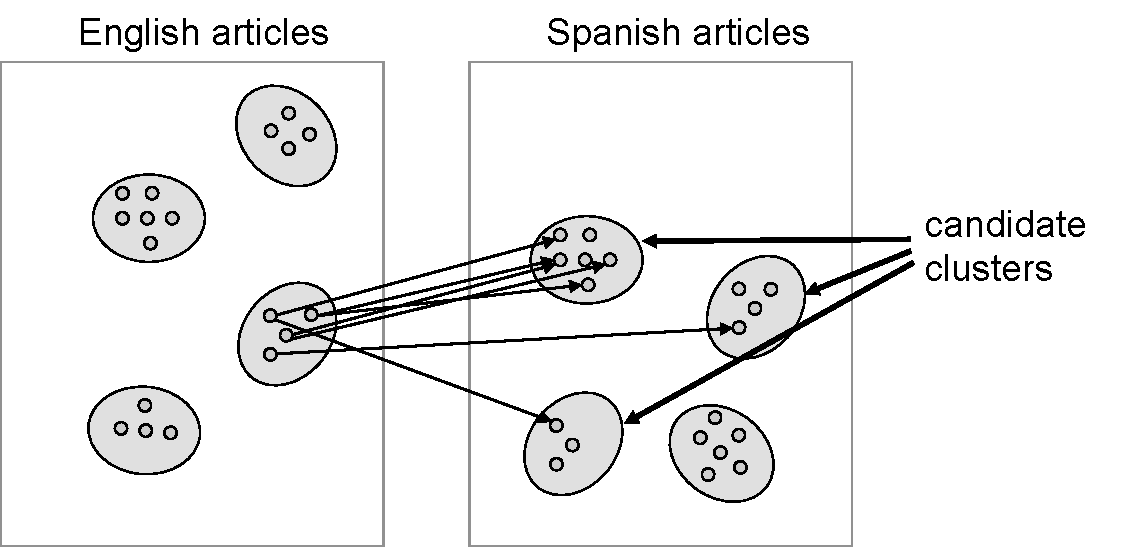
\includegraphics[width=0.7\textwidth]{figures/clusters.pdf}
\caption[Cluster linking]{Clusters composed of English and Spanish news articles. Arrows link English articles with their Spanish $k$-nearest neighbor matches according to the cross-lingual similarity.}
\label{fig:clusters}
\end{figure}

Matching of clusters is a \emph{generalized matching} problem. We cannot assume that there is only
one cluster per language per event, nor can we assume complete coverage -- i.e., that there exists
at least one cluster per event in every language. This is partly due to news coverage which might
be more granular in some languages, partly due to noise and errors in the event detection process. This
implies that we cannot make assumptions on the matching (e.g., one-to-one or complete matching) and excludes
the use of standard weighted bipartite matching type of algorithms for this problem. An example is shown in
Figure~\ref{fig:clusters}, where a cluster may contain articles which are closely matched with many clusters in a different language.

We also seek an algorithm which does not do exhaustive comparison of all clusters, since that can become prohibitively expensive when working in a real-time setting. More specifically, we wish to avoid testing cluster $c_i$ with all the clusters from all the other languages. Performing exhaustive comparison would result in $O(|C|^2)$ tests, where $|C|$ is the number of all clusters (over all languages), which is not feasible when the number of clusters is on the order of tens of thousands. We address this by testing only clusters that are connected with at least one $k$-nearest neighbor (marked as \emph{candidate clusters} in Figure~\ref{fig:clusters}).

\section{Algorithm}\label{algo:features}

In order to identify clusters that are equivalent to cluster $c_i$, we have developed
a novel two-stage approach. For a cluster $c_i$, we first efficiently identify a small set of
candidate clusters and then find those clusters among the candidates, which are
equivalent to $c_i$. An example is  shown in  Figure~\ref{fig:clusters}.

The details of the first step are described in Algorithm~\ref{cluster_merge_algo1}. The algorithm
begins by individually inspecting each news article $a_i$ in the cluster $c_i$. Using a chosen
method for computing cross-lingual document similarity (see Chapter~\ref{chap:crosslingual}), it identifies
the ten\footnote{This parameter was manually selected based on the storage and speed requirements of a real system.}
most similar news articles to $a_i$ in each language $\ell \in L$. For each similar
article $a_j$, we identify its corresponding  cluster $c_j$ and add it to the set of candidates.
The set of candidate clusters obtained in this way is several orders of magnitude smaller than the
number of all clusters, and at most linear with respect to the number of news articles in
cluster $c_i$. In practice, clusters contain highly related articles and as such similar
articles from other languages mostly fall in only a few candidate clusters.

Although computed document similarities are approximate, our  assumption is that articles
in different languages describing the same event will generally have a higher similarity
than articles about different events. While this assumption does not always hold, redundancy
in the data should mitigate these false positives.

\begin{algorithm}[t!]
\SetKwInput{KwInput}{input}\SetKwInput{KwOutput}{output}
\KwInput{test cluster $c_i$, a set of clusters $C_\ell$ for each language $\ell \in L$}
\KwOutput{a set of clusters $C$ that are potentially equivalent to $c_i$}
$C \leftarrow \{\}$\;
\For{article $a_i \in c_i$} {
    \For{language $\ell \in L$} {
        \tcc{use hub CCA to find 10 most similar articles to article $a_i$ in language $\ell$}
        $SimilarArticles = getCCASimilarArticles(a_i, \ell)$\;
        \For{article $a_j \in SimilarArticles$} {
            \tcc{find cluster $c_j$ to which article $a_j$ is assigned to}
            $c_j \leftarrow c$, such that $c \in C_\ell$ and $a_j \in c$\;
            \tcc{add cluster $c_j$ to the set of candidates $C$}
            $C \leftarrow C \cup \{ c_j \}$\;
        }
    }
}
\caption[Algorithm for identifying candidate clusters]{Algorithm for identifying candidate clusters $C$ that are potentially equivalent to $c_i$}
\label{cluster_merge_algo1}
\end{algorithm}

The second stage of the algorithm determines which (if any) of the candidate clusters are equivalent to $c_i$.
We treat this task as a supervised learning problem. For each candidate cluster $c_j \in C$, we compute
a vector of learning features that should be indicative of whether $c_i$ and $c_j$ are equivalent or not
and apply a binary classification model that predicts if the clusters are equivalent or not. The classification
algorithm that we used to train a model was a linear Support Vector Machine (SVM) method~\cite{shawe-taylor04kernel}.

We use three groups of features to describe a cluster pair $(c_i, c_j)$. The first group is based
on {\bf cross-lingual article links}, which are derived using cross-lingual similarity:
each news article $a_i$ is linked with its $10$-nearest neighbors articles from all other
languages (ten per each language). The group contains the following features:

\begin{itemize}
\item \texttt{linkCount} is the number of times any of the news articles from $c_j$ is among $10$-nearest neighbors for articles from $c_i$. In other words, it is the number of times an article from $c_i$ has a very similar article (i.e., is among 10 most similar) in $c_j$.
\item \texttt{avgSimScore} is the average similarity score of the links, as identified for \texttt{linkCount}, between the two clusters.
\end{itemize}

The second group are {\bf concept-related features}. Articles that are imported into Event Registry
are annotated by disambiguating mentioned \emph{entities} and \emph{keywords} to the corresponding
Wikipedia pages~\cite{zhang2014}. Whenever ``David Bowie'' is, for example, mentioned in the article,
the article is annotated with a link to his Wikipedia page. In the same way, all mentions of
entities (people, locations, organizations) and ordinary keywords (e.g., ``bank'', ``tax'', ``ebola'', ``plane'', ``company'')
are annotated. Although the Spanish article about ``Bowie'' will be annotated with his Spanish
version of the Wikipedia page, in many cases we can link the Wikipedia pages to their English
versions. This can be done since Wikipedia itself provides information regarding which pages
in different languages represent the same concept/entity. Using this approach, the word ``avi\'on''
in a Spanish article will be annotated with the same concept as the word ``plane'' in an English article.
Although the articles are in different languages, the annotations can therefore provide a language-independent
vocabulary that can be used to compare articles/clusters. By analyzing all the articles in
clusters $c_i$ and $c_j$, we can identify the most relevant entities and keywords for each cluster.
Additionally, we can also assign weights to the concepts based on how frequently they occur in the
articles in the cluster. From the list of relevant concepts and corresponding weights, we consider
the following features:

\begin{itemize}
\item \texttt{entityCosSim} is the cosine similarity between vectors of entities from clusters $c_i$ and $c_j$.
\item \texttt{keywordCosSim} is the cosine similarity between vectors of keywords from clusters $c_i$ and $c_j$.
\item \texttt{entityJaccardSim} is  Jaccard similarity coefficient~\cite{levandowsky1971} between sets of entities from clusters $c_i$ and $c_j$.
\item \texttt{keywordJaccardSim} is  Jaccard similarity coefficient between sets of keywords from clusters $c_i$ and $c_j$.
\end{itemize}

The last group of features contains three {\bf miscellaneous features} that seem
discriminative but are unrelated to the previous two groups:
\begin{itemize}
\item \texttt{hasSameLocation} feature is a boolean variable that is true when the location of the event
in both clusters is the same. The location of events is estimated by considering the locations mentioned
in the articles that form a cluster and is provided by Event Registry.
\item \texttt{timeDiff} is the absolute difference in hours between the two events. The publication time
and date of the events is computed as the average publication time and date of all the articles and is
provided by Event Registry.
\item \texttt{sharedDates} is determined as the Jaccard similarity coefficient between sets of date
mentions extracted from articles. We use extracted mentions of dates provided by Event Registry, which
uses an extensive set of regular expressions to detect and normalize mentions of dates in different forms.
\end{itemize}

